\section{Models and Methods} \label{sec:models-and-methods}
In this section we describe data pre-processing techniques, model architectures and the post-processing methods that we apply to our model outputs.

\subsection{Baseline} \label{subsec:baseline}
For our baseline model, we split each of our images and masks in disjoint patches of size $16 \times 16$. We then normalize each image patch by subtracting the mean and dividing by the standard deviation across our training set. To compute the patch label, we compute the mean across the mask patch and set the label to $1$ (road) if the mean is bigger than $0.25$ and $0$ (not road) otherwise.

These patches are used to train a convolutional neural network. The exact architecture is described in \autoref{tab:baseline}.

\begin{table}[h]
    \centering
    \begin{tabular}{|c|c|c|}
        \hline
        Conv(filters=$32$, kernel=$5 \times 5$) & MaxPool(kernel=$2 \times 2$) & BatchNorm \\
        \hline
        \hline
        Conv(filters=$64$, kernel=$5 \times 5$) & MaxPool(kernel=$2 \times 2$) & BatchNorm \\
        \hline
        \hline
        Dense(units=$512$, activ.=ReLU) & BatchNorm &  \\
        \hline
        \hline
        Dense(units=$1$, activ.=Sigmoid) & & \\
        \hline
    \end{tabular}
    \caption{Architecture of our baseline CNN model.}
    \label{tab:baseline}
\end{table}

\subsection{Improved Baseline} \label{subsec:better-baseline}
Here we borrow from the ideas presented in \cite{Mni10}. We use a much bigger patch of size $64 \times 64$ to predict the middle $16 \times 16$ patch. This gives our model more information and hence a better prediction is expected. Similarly to \autoref{subsec:baseline}, we split each image in disjoint patches of size $64 \times 64$, using $0$ padding on the edges. Image patch normalization, mask patch extraction and label computation are identical to what we did in \autoref{subsec:baseline}.

To predict the labels, we use a convolutional neural network. The exact architecture is described in \autoref{tab:better-baseline}.

\begin{table}[h]
    \centering
    \begin{tabular}{|c|c|c|}
        \hline
        Conv(filters=$32$, kernel=$3 \times 3$) & MaxPool(kernel=$2 \times 2$) & BatchNorm \\
        \hline
        \hline
        Conv(filters=$64$, kernel=$3 \times 3$) & MaxPool(kernel=$2 \times 2$) & BatchNorm \\
        \hline
        \hline
        Conv(filters=$64$, kernel=$3 \times 3$) & MaxPool(kernel=$2 \times 2$) & BatchNorm \\
        \hline
        \hline
        Conv(filters=$128$, kernel=$3 \times 3$) & MaxPool(kernel=$2 \times 2$) &BatchNorm \\
        \hline
        \hline
        Dense(units=$512$, activ.=ReLU) & BatchNorm &  \\
        \hline
        \hline
        Dense(units=$1$, activ.=Sigmoid) & & \\
        \hline
    \end{tabular}
    \caption{Architecture of our improved baseline CNN model.}
    \label{tab:better-baseline}
\end{table}

After obtaining the results from the CNN we tried incorporating the continuous road structure in our prediction. We group our labels into $7 \times 7$ patches and use these groupings to refine the prediction of the middle label.

We use an SVM with a radial basis function kernel as our post processing model. This is different from what was done in \cite{He15} where a CNN was used.

\subsection{UNet} \label{subsec:UNet}
Our best performing models in this task are fully convolutional networks, which make use of only convolutional and sampling (down \& up) layers to obtain outputs with the same spatial dimensions as the input. First, we try UNet as introduced in \cite{Ron15}. One of the advantages of these type of networks is that they don't need enormous amounts of data to yield excellent results.

\begin{figure}[h]
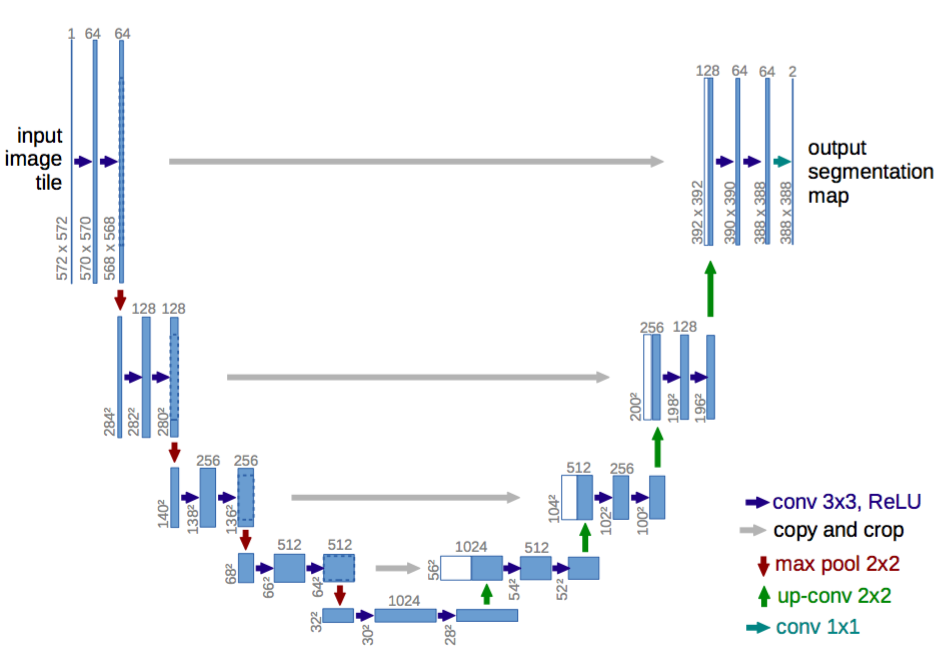
\includegraphics[width=8cm]{images/unet.png}
\caption{Auto-encoder approach using UNet. Image taken from \cite{Ron15}}
\end{figure}

Contrary to the baseline models, we can feed the entire image to the network and backpropagate the loss from the entire mask. Nevertheless, some pre-processing is necessary. We scale all our images to the $[0,1]$ interval and normalize the data with the channel-wise mean and standard deviation of the ImageNet \cite{Imagenet} dataset. This type of normalization is necessary because we use a model pre-trained on this particular dataset. The data is further augmented with random rotations, flips, crops and scaling.

Being highly flexible, UNet allows us to try different CNN architectures in its contracting and expanding paths. Among the ones we experimented with were: VGG \cite{Zis14} and ResNet \cite{He15}.

The masks generated by the network needed further processing in order to convert them into $16 \times 16$ patch predictions. We tried averaging the model output directly in each patch and applying a threshold or applying the threshold twice, once on the pixel level and once on the mask patch average level.

\subsection{FCN and DeepLabV3} \label{subsec:fcn-deeplab}
The most successful models among the ones we experimented with were the FCN \cite{Lon14} and DeepLabV3 \cite{Che17} based ones. 

The preprocessing part is identical to \autoref{subsec:UNet}, except for the normalization stage. The models we use, are pre-trained on the MS-COCO \cite{Coco} dataset and this forces us to subtract the channel-wise mean and standard deviation from this dataset. Additionally, we augment the images as we observe that these models are prone to over-fitting. We apply random rotations, horizontal and vertical flipping, as well as random jittering in the color space, contrast, brightness etc.

FCN and DeepLabV3 are also very flexible. We could choose from several CNN architectures in the contracting and expanding paths, pre-trained on different datasets. However, we experimented only with the ResNet variants as they proved easier to train.

\begin{figure}[h]
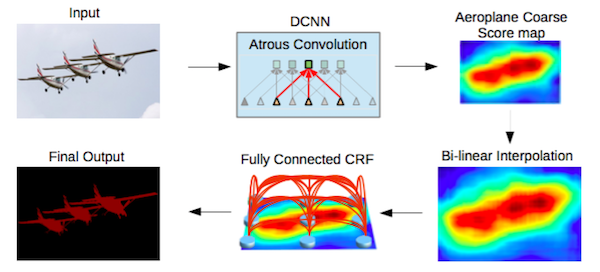
\includegraphics[width=8cm]{images/deeplabv2.png}
\caption{A simplistic overview of DeepLab architecture. Image taken \cite{Che17}.}
\end{figure}

\subsection{FCN Ensemble} \label{subsec:ensemble}
In order to further improve our performance, we finally create a simple ensemble using FCN and DeepLabV3 with ResNet 101 backbones each. The preprocessing part is identical to \autoref{subsec:fcn-deeplab}. The final output is a normalized linear combination of the two models, which is then trained against the target masks.
